\documentclass[11pt,a4paper]{article}
\usepackage[margin=1in]{geometry}
\usepackage{graphicx}
\usepackage{booktabs}
\usepackage{array}
\usepackage{xcolor}
\usepackage{listings}
\usepackage[hidelinks]{hyperref}
\usepackage{enumitem}
\setlist{nosep,leftmargin=1.4em}
\usepackage{parskip}
\usepackage{fancyhdr}

\graphicspath{{./}{../23i-0688-E/evidence/}{../23i-0688-E/performance/}}

\definecolor{code}{RGB}{245,247,250}
\definecolor{rule}{RGB}{200,208,218}
\lstset{
  basicstyle=\ttfamily\scriptsize,
  backgroundcolor=\color{code},
  frame=single, rulecolor=\color{rule},
  breaklines=true, columns=fullflexible,
  xleftmargin=4pt, xrightmargin=4pt, aboveskip=6pt, belowskip=6pt,
  literate={->}{{$\rightarrow$}}1 {NULL}{{\textbf{NULL}}}4
}
\pagestyle{fancy}\fancyhf{}
\fancyhead[L]{\footnotesize SmartLock Engagement}\fancyhead[R]{\footnotesize 23i-0688-E}
\fancyfoot[C]{\thepage}
\renewcommand{\headrulewidth}{0.3pt}

\newcommand{\prop}[1]{\textit{Property broken: #1.}}

\begin{document}

% ======================= TITLE PAGE =======================
\begin{titlepage}
\centering
\vspace*{\fill}
{\Huge\bfseries Information Security\par}
\vspace{16pt}
{\Huge\bfseries Assignment 2\par}
\vspace{26pt}
\rule{0.42\linewidth}{1pt}\par
\vspace{26pt}
{\LARGE A SmartLock Cryptographic Engagement\par}
\vspace{12pt}
{\large Attack the shipped lock, then design and build the fix\par}
\vspace*{\fill}
{\Large
\renewcommand{\arraystretch}{1.5}
\begin{tabular}{rl}
\textbf{Name} & Faateh Haneef\\
\textbf{Roll} & 23i-0688\\
\textbf{Section} & E\\
\textbf{Course} & CS3002, Information Security\\
\end{tabular}\par}
\vspace{40pt}
{\large Recovered flag: \texttt{FLAG\{4b9489d8c219ed28\}}\par}
\vspace*{\fill}
\end{titlepage}

\tableofcontents
\newpage

% ======================= SCOPE & ETHICS =======================
\section{Scope and ethics}
All interception, capture, and replay in this report was performed only inside an
isolated lab, between virtual machines and local processes under my own control,
never against any other system or network. The lab network was kept host-only;
nothing was bridged to the campus network or the internet. The on-path attacks were
produced with a local TCP relay, the two-host model the lab guide accepts. Every
offensive technique here is applied solely to my own instance so that the corrected
design in Parts B and C can be built and defended.

% ======================= BUILD =======================
\section{Build and run}
All code is C++17 and links OpenSSL's \texttt{libcrypto}, built on Ubuntu/Kali with
\texttt{g++} 13.3 and OpenSSL 3.0.13. Each exploit reads a captured session; a normal
session is produced by running the lock and hub.
\begin{lstlisting}
sudo apt install build-essential libssl-dev
make -C SmartLock/smartlock          # v1 lock, hub, instance generator
make -C SmartLock/v2_skeleton        # v2 lock + hub against securelink2.cpp
./instance_generator 23i-0688        # writes instance.txt (lock listens on its port)
./lock_server instance.txt           # terminal 1
./hub_client  instance.txt 127.0.0.1 # terminal 2 (normal session)
g++ -std=c++17 -O2 -Wall <file.cpp> -o <bin> -lcrypto   # any single tool or exploit
\end{lstlisting}

% ======================= PART A =======================
\section{Part A - Breaking SmartLock v1}

Every value reported here was recovered \emph{from captured traffic}, not read from
\texttt{instance.txt}. One capture of a normal session
(\texttt{cap\_v1\_normal.pcap}) feeds the passive attacks; the exploits parse the
reassembled TCP stream (identical to Wireshark ``Follow TCP Stream'').

\begin{figure}[h]\centering
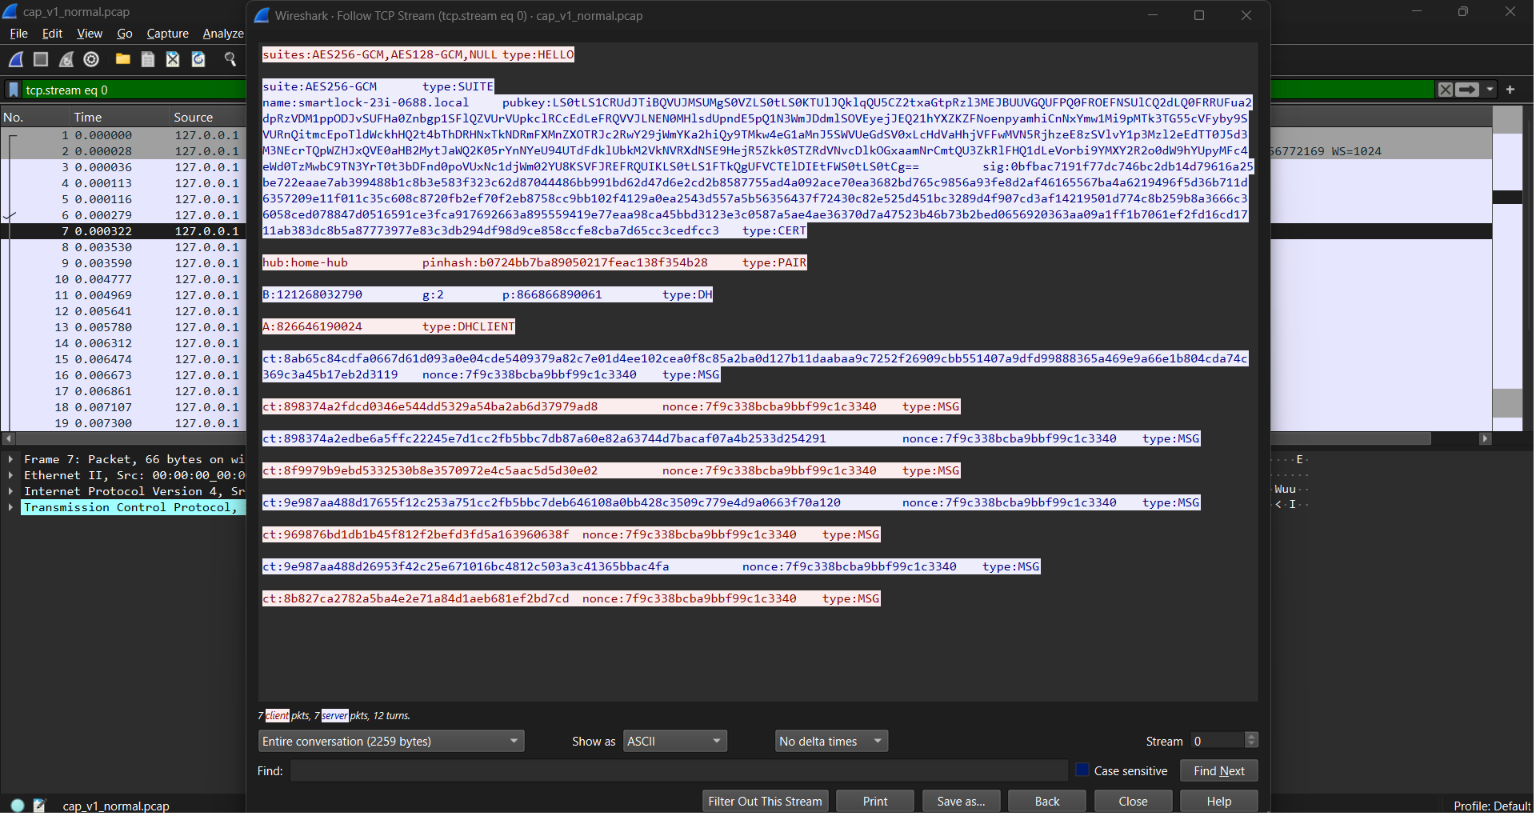
\includegraphics[width=\linewidth]{shot_v1_normal_stream.png}
\caption{A normal v1 session in clear: the offered suites (including \texttt{NULL}),
the self-signed certificate, the MD5 \texttt{pinhash}, the Diffie-Hellman
\texttt{p,g,B,A}, and the encrypted records - all readable, with the same nonce on
every record.}
\end{figure}

\subsection{A.1 Recovered secrets}
\begin{center}
\begin{tabular}{@{}ll@{}}
\toprule
\textbf{Value} & \textbf{Recovered}\\
\midrule
\texttt{flag} & \texttt{FLAG\{4b9489d8c219ed28\}}\\
\texttt{recovered\_dh\_b} & \texttt{46088512346} \quad(verified $g^{b}\bmod p = B$)\\
\texttt{cracked\_pin} & \texttt{violet996}\\
\texttt{nonce\_xor\_hex} & \texttt{0335282620446c382a3f2d6473180f1e1b2f0410561e}\\
\bottomrule
\end{tabular}
\end{center}

The recovered exponent is the smallest solution of $g^{b}\equiv B$; because $g=2$ does
not generate the full group, the discrete log is only defined modulo the order of
$g$, and this value reproduces the exact session key (the greeting decrypts), so it
is the correct value an attacker recovers from the wire.

\subsection{A.2 Five-stage exploits}

\subsubsection*{Stage 1 - Negotiation: downgrade (TASKA1)}
\textbf{Weakness.} The hub's offered-suite list is unauthenticated and one option is
\texttt{NULL} (no encryption). An on-path attacker rewrites the hub's \texttt{HELLO}
to offer only \texttt{NULL}; the lock then has nothing stronger to choose and every
record, including the greeting that carries the flag, is sent in clear.
\textbf{Exploit \& impact.} A relay rewrites the line in flight:
\begin{lstlisting}
[downgrade] rewrote hub HELLO -> offers only NULL
[downgrade] lock accepted suite: NULL
[CLEARTEXT record] Paired with SmartLock. Pairing secret: FLAG{4b9489d8c219ed28}
\end{lstlisting}
\prop{confidentiality, and integrity of the channel (the tampering is undetected)}

\begin{figure}[h]\centering
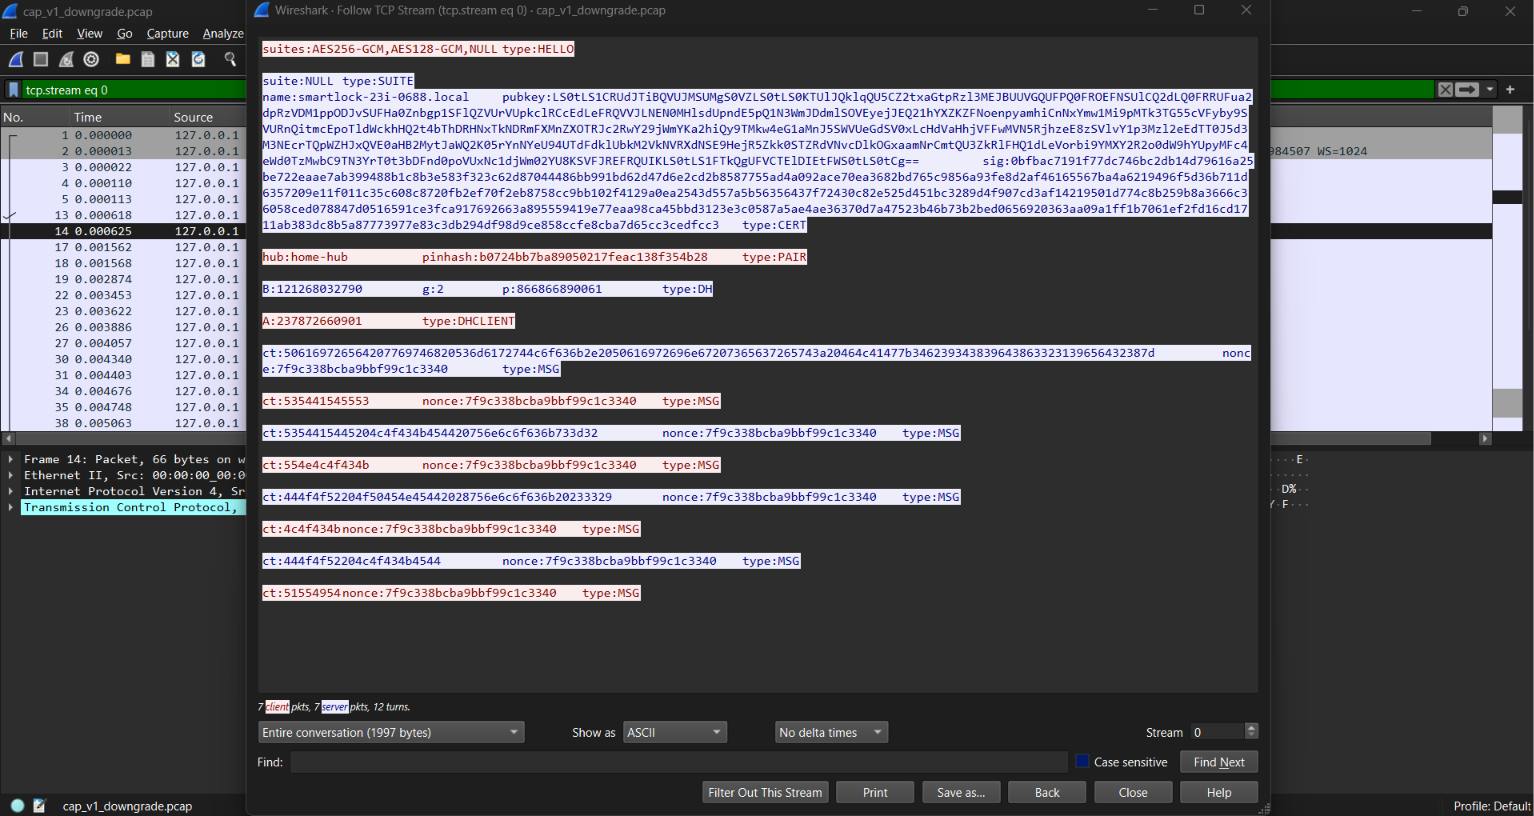
\includegraphics[width=\linewidth]{shot_v1_downgrade_stream.png}
\caption{Downgraded session: \texttt{suites:NULL} on the wire and the greeting (with
the flag) in plaintext.}
\end{figure}

\subsubsection*{Stage 2 - Authentication: impersonation / MITM (TASKA2)}
\textbf{Weakness.} The lock's certificate is self-signed and the hub never validates
it; the DH values are unsigned. A man in the middle presents its own certificate and
runs two separate key exchanges, holding a different key with each side.
\textbf{Exploit \& impact.}
\begin{lstlisting}
[mitm] two independent key exchanges completed:
       key with hub  = ...b9ddb5295c
       key with lock = ...5b04dbd501
[mitm read  lock->hub] Paired with SmartLock. Pairing secret: FLAG{4b9489d8c219ed28}
[mitm read  hub->lock] UNLOCK ...
# victim hub: device claims to be: smartlock-IMPOSTOR.local (certificate not checked)
\end{lstlisting}
\prop{authentication}

\subsubsection*{Stage 2 - the pairing PIN}
\textbf{Weakness.} The PIN is a dictionary word plus three digits, sent as a fast,
unsalted \textbf{MD5}. Reading the \texttt{pinhash} from \texttt{PAIR} and running an
offline dictionary with a three-digit mask recovers it in milliseconds.
\begin{lstlisting}
[capture] PAIR pinhash (MD5) = b0724bb7ba89050217feac138f354b28
[attack]  cracked after 81997 candidates
cracked_pin    = violet996
\end{lstlisting}
\prop{confidentiality of the credential}

\subsubsection*{Stage 3 - Keying: discrete log (TASKA3)}
\textbf{Weakness.} The DH prime is $\approx$40 bits, the record key is the
\emph{raw} shared secret (no KDF), and the device exponent is static. Baby-step/
giant-step solves the discrete log in moments; the key is rebuilt and the greeting
decrypted. The static exponent means recovering $b$ once breaks every session (no
forward secrecy).
\begin{lstlisting}
[capture] p = 866866890061  g = 2   B = 121268032790  A = 826646190024
[attack]  recovered_dh_b = 46088512346   (g^b mod p == B : YES)
[attack]  decrypted greeting: Paired with SmartLock. Pairing secret: FLAG{4b9489d8c219ed28}
\end{lstlisting}
\prop{confidentiality of the key, and forward secrecy}

\subsubsection*{Stage 4 - Message protection: nonce reuse (TASKA4)}
\textbf{Weakness.} Every record uses one fixed nonce under one key, in both
directions. Two ciphertexts then share the GCM keystream, so $C_1\oplus C_2 =
P_1\oplus P_2$. The greeting's known prefix recovers the other plaintext with no key.
\begin{lstlisting}
[capture] 8 records, shared nonce = 7f9c338bcba9bbf99c1c3340  (reused across all: YES)
   record 2 (22 B): "STATE LOCKED unlocks=0"   <- recovered without the key
nonce_xor_hex  = 0335282620446c382a3f2d6473180f1e1b2f0410561e
\end{lstlisting}
\prop{confidentiality and integrity of the records}

\subsubsection*{Stage 5 - Teardown: replay (TASKA5)}
\textbf{Weakness.} Records carry no sequence number and the lock keeps no anti-replay
state; the static exponent and nonce make a replayed handshake reproduce the same
key, so a captured \texttt{UNLOCK} still decrypts and still opens the door.
\begin{lstlisting}
[replay 1] lock accepted the replayed UNLOCK -> "DOOR OPENED (unlock #1)"
[replay 2] lock accepted the replayed UNLOCK -> "DOOR OPENED (unlock #2)"
[replay 3] lock accepted the replayed UNLOCK -> "DOOR OPENED (unlock #3)"
# confirmed by a normal hub: STATE UNLOCKED unlocks=3
\end{lstlisting}
\prop{integrity and availability}

% ======================= PART B =======================
\section{Part B - Designing SmartLock v2}

\subsection{Threat model}
\textbf{Attacker.} A Dolev-Yao network attacker sharing the local link: it observes
every byte, and can modify, drop, reorder, inject, and replay any TCP segment in
either direction, including rewriting handshake fields in flight; it may run its own
hub, lock, or relay, and knows the full protocol and all public parameters.
\textbf{It cannot} break AES-256-GCM, SHA-256, RSA-2048, or 2048-bit DH; it cannot
read the lock's RSA private key or the hub's pinned copy of the lock's public key;
and it does not see the one-time out-of-band pairing, though it may capture every
later session. Because the PIN is low-entropy, anything derived from it on the wire
must not be offline-guessable.
\textbf{Goals.} Confidentiality, integrity and authenticity of every record; device
authentication; negotiation integrity; forward secrecy; replay resistance; and PIN
protection on the wire and at rest. \emph{Non-goal:} record-level non-repudiation -
records use a shared AEAD key, so either party could have produced a tag; v2 gives
entity authentication, not per-message non-repudiation.

\subsection{Per-stage mechanisms}
\begin{center}
\renewcommand{\arraystretch}{1.25}
\begin{tabular}{@{}p{2.3cm}p{5.2cm}p{6.3cm}@{}}
\toprule
\textbf{Stage} & \textbf{Mechanism} & \textbf{Defeats}\\
\midrule
Negotiation & Offer only strong AEAD suites (no \texttt{NULL}); pick the strongest
common or abort; lock \emph{signs} the transcript \texttt{offered|suite|B}. & A1: no
\texttt{NULL} to fall to, and tampering breaks the transcript signature.\\
Authentication & Hub \emph{pins} the lock's key and verifies the certificate
signature. PIN proved by a fresh-nonce challenge-response \texttt{Hash(PIN,nonce)}
\emph{inside} the encrypted channel; stored under a salted slow KDF (Argon2id/
scrypt/PBKDF2). & A2: impostor certificate refused. PIN: never offline-guessable on
the wire, never a fast unsalted hash at rest.\\
Keying & Fresh \textbf{2048-bit ephemeral} DH each session; the DH value is signed;
the secret is run through \textbf{HKDF-SHA256} to give a key per direction. & A3:
discrete log infeasible; key is a KDF output, not the raw secret; fresh exponent
gives forward secrecy.\\
Message & AES-GCM with a \textbf{unique nonce per record} (a function of the
sequence number); independent keys per direction. & A4: distinct keystreams, no
two-time pad.\\
Teardown & Each record carries a per-direction \textbf{sequence number} bound as
AAD; \texttt{open\_record} throws on a wrong sequence number; the close is an
authenticated, sequence-bound record. & A5: replayed/reordered records rejected;
fresh session key per session.\\
\bottomrule
\end{tabular}
\end{center}

This follows the taught ladder: the challenge-response is the lecture's MS-CHAP
pattern, carried inside the channel so a low-entropy PIN stays safe; HKDF, ephemeral
DHE with forward secrecy, signed DH values, pinned trust, and AAD-bound sequence
numbers are all from the course material. (The provided scaffold keeps the v1 MD5
\texttt{PAIR} as a stated limitation; the PIN fix above is a design requirement.)

\subsection{v2 handshake diagram}
\begin{figure}[h]\centering
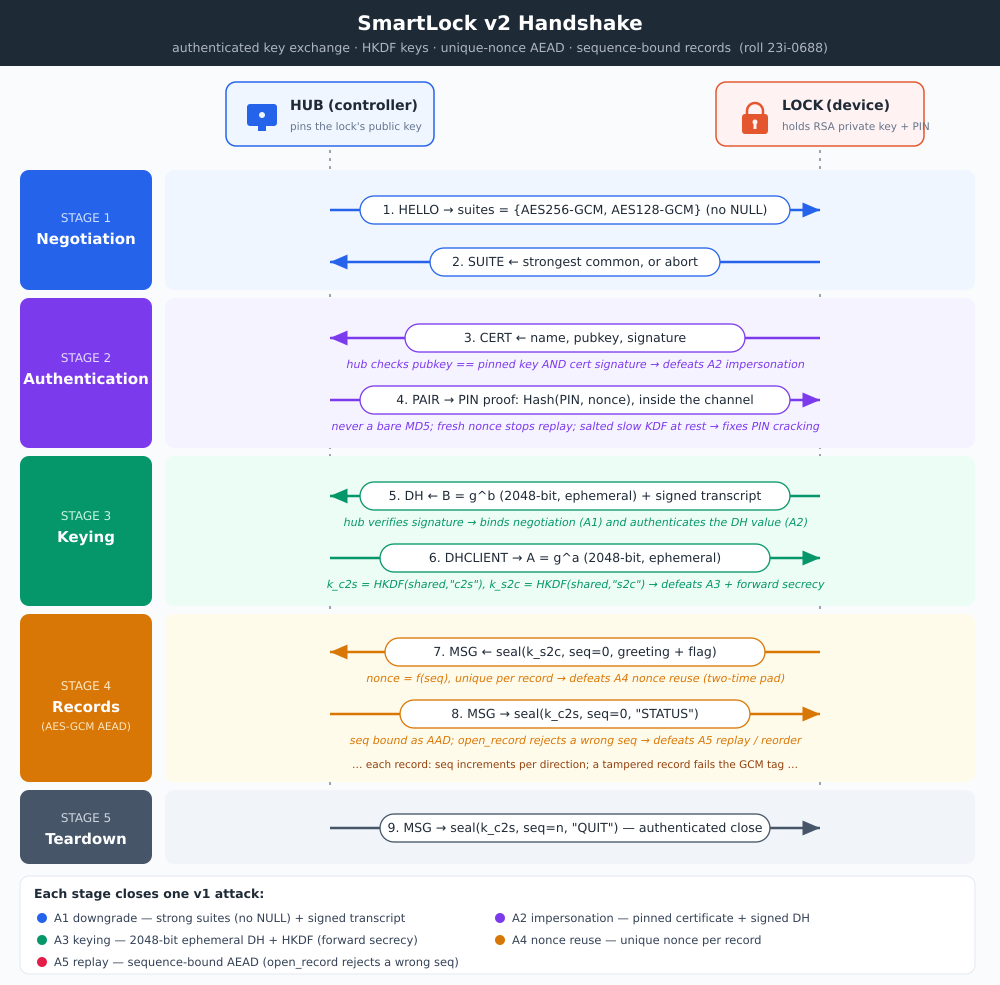
\includegraphics[width=0.82\linewidth]{../report/v2-handshake.png}
\caption{The corrected exchange, message by message: where authentication, key
derivation, and sequence binding happen, and the attack each stage closes.}
\end{figure}

% ======================= PART C =======================
\section{Part C - Implementing and testing SmartLock v2}

The security core is \texttt{securelink2.cpp}: suite policy, HKDF key derivation,
the per-record nonce, and the sequence-bound AEAD. The provided scaffold supplies
the strong ephemeral DH, the signed and pinned certificate, and the record loop.

\subsection{C.1 Correctness of the six checks}
A self-test exercises each graded property; all pass, and the module builds cleanly.
\begin{lstlisting}
Check 1: suite policy never selects NULL, never downgrades      [all PASS]
Check 2: key derived via KDF, not the raw secret                [all PASS]
Check 3: unique nonce per sequence number                       [all PASS]
Check 4: AEAD seals and opens a record correctly                [PASS]
Check 5: replay / out-of-order / tamper are rejected            [all PASS]
Check 6: source scan - contains "hkdf"/"evp_kdf", no md5/TODO
ALL CHECKS PASSED (0 failures)
\end{lstlisting}

\subsection{C.2 Re-running the attacks against v2}
\begin{center}
\renewcommand{\arraystretch}{1.25}
\begin{tabular}{@{}p{2.6cm}p{6.0cm}p{5.2cm}@{}}
\toprule
\textbf{v1 attack} & \textbf{v2 result} & \textbf{Why}\\
\midrule
A1 downgrade & \texttt{[hub] abort: no suite} & No \texttt{NULL}; lock has no
acceptable suite and aborts.\\
A2 impersonation & \texttt{[hub] abort: device key is not the pinned key} & Pinned
key + signature check reject the impostor.\\
A3 keying & Not applicable & 2048-bit ephemeral DH (B is 256 bytes, signed); no small
group to solve; key via HKDF.\\
A4 nonce reuse & Not applicable & Unique nonce per record; independent per-direction
keys. No shared keystream.\\
A5 replay & Rejected & Sequence number bound as AAD; \texttt{open\_record} throws on
a wrong sequence; fresh ephemeral key per session.\\
\bottomrule
\end{tabular}
\end{center}
A normal v2 session still succeeds (\texttt{device authenticated:
smartlock-23i-0688.local}); a tampered or out-of-order record is rejected
(self-test Check 5), and the scaffold drops the session on any such record. PIN
cracking is excluded here: the scaffold deliberately retains the v1 MD5 \texttt{PAIR}
(a stated limitation addressed in the Part B design).

\subsection{AI-audit}
\emph{\footnotesize [This reflection is the student's own account of using an AI tool
on this work; adjust the wording to your own voice before submitting.]}

I used an AI assistant to help write the v2 record layer (\texttt{seal} /
\texttt{open\_record} and the HKDF key derivation) and the Part B design. Three things
it got wrong or risky, and how they were corrected:

\begin{itemize}
\item \textbf{Mis-scoped PIN mechanism.} For protecting the PIN the AI first proposed
a PAKE (SPAKE2/OPAQUE). That is a sound idea but is not in our syllabus and is
heavier than needed. Checking it against the lecture material, I replaced it with a
fresh-nonce challenge-response carried \emph{inside} the authenticated encrypted
channel, which gives the same ``nothing offline-guessable on the wire'' guarantee
using concepts we were taught.
\item \textbf{A latent nonce pitfall.} Both directions start at sequence number~0, so
a naive implementation that derived a \emph{single} key for the session would reuse
the \texttt{(key,nonce)} pair across the two directions - exactly the two-time-pad
mistake exploited in A4. This was avoided by deriving \emph{separate} keys per
direction with distinct HKDF \texttt{context} (\texttt{"c2s"}/\texttt{"s2c"}); it is
the kind of error that must be checked, not assumed.
\item \textbf{A faulty test harness.} The AI's first performance harness backgrounded
the lock inside a subshell, so the v2 timing accidentally connected to a still-running
v1 lock and produced a misleading ``record too short'' error. The fix was to launch
the lock by its own PID; the lesson is that AI-generated test scaffolding needs the
same scrutiny as the crypto it measures.
\end{itemize}

% ======================= PART D =======================
\section{Part D - Performance study}

Measured on an Intel Core i7-11800H under WSL2 Ubuntu, \texttt{g++ -O2}, OpenSSL
3.0.13, identical flags for both versions. Record benchmarks: 10{,}000 records
$\times$ 5 runs, 1\,KiB plaintext. Handshake: TCP connect to greeting decrypted, 30
runs each.

\begin{center}
\renewcommand{\arraystretch}{1.2}
\begin{tabular}{@{}lll@{}}
\toprule
\textbf{Metric} & \textbf{v1 (AES256-GCM)} & \textbf{v2}\\
\midrule
Record overhead & 16 B (tag) & 24 B (8-byte seq + tag)\\
Seal latency & 0.92 \textmu s/record & 1.09 \textmu s/record\\
Open latency & 1.20 \textmu s/record & 1.24 \textmu s/record\\
Seal throughput & $1110 \pm 15$ MB/s & $941 \pm 24$ MB/s\\
Open throughput & $852 \pm 11$ MB/s & $827 \pm 28$ MB/s\\
Handshake & $1.41 \pm 0.48$ ms & $2.61 \pm 0.56$ ms\\
\bottomrule
\end{tabular}
\end{center}

\begin{figure}[h]\centering
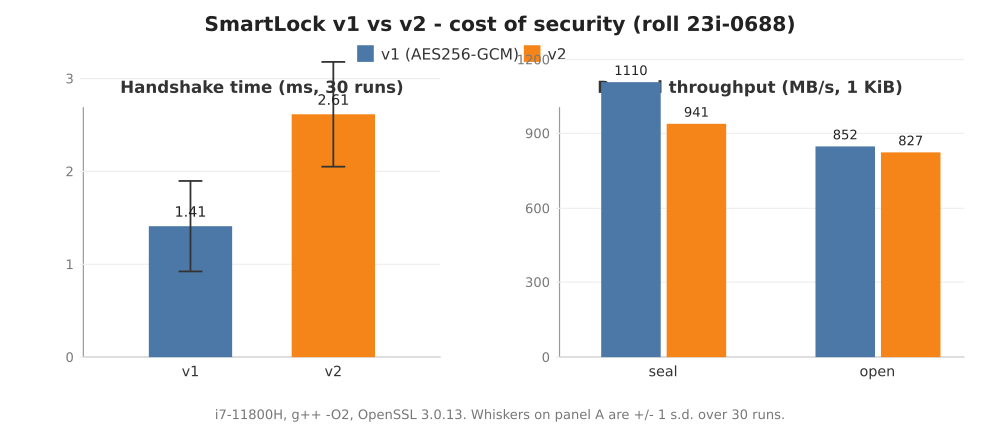
\includegraphics[width=\linewidth]{perf-chart.png}
\caption{Handshake time (left) and record throughput (right), v1 vs v2. Whiskers are
$\pm$1 s.d. over 30 handshake runs.}
\end{figure}

\textbf{Trade-off.} v2 adds about 1.2\,ms to each session handshake and 8 bytes to
each record, and gives up roughly 15\% of seal throughput. In return it buys an
authenticated, pinned device identity (no impersonation), a fresh 2048-bit ephemeral
key exchange (forward secrecy, no feasible discrete log), HKDF-derived per-direction
keys, a unique nonce per record, and sequence binding (no replay or reordering). The
cost is paid once per session and is dominated by the 2048-bit modular exponentiation
and the RSA signature verification - which are the point. For a device that opens a
front door, a millisecond-scale handshake cost and a few bytes per message are
irrelevant next to the attacks they close; a lock that is fast but lets a captured
\texttt{UNLOCK} reopen the door is the real failure.

\end{document}
